%iffalse
\documentclass[journal]{IEEEtran}
\usepackage[a5paper, margin=10mm, onecolumn]{geometry}
%\usepackage{lmodern} % Ensure lmodern is loaded for pdflatex
\usepackage{tfrupee} % Include tfrupee package

\setlength{\headheight}{1cm} % Set the height of the header box
\setlength{\headsep}{0mm}     % Set the distance between the header box and the top of the text

\usepackage{gvv-book}
\usepackage{gvv}
\usepackage{cite}
\usepackage{amsmath,amssymb,amsfonts,amsthm}
\usepackage{algorithmic}
\usepackage{graphicx}
\usepackage{textcomp}
\usepackage{xcolor}
\usepackage{txfonts}
\usepackage{listings}
\usepackage{enumitem}
\usepackage{mathtools}
\usepackage{gensymb}
\usepackage{comment}
\usepackage[breaklinks=true]{hyperref}
\usepackage{tkz-euclide} 
\usepackage{listings}
% \usepackage{gvv}                                        
\def\inputGnumericTable{}                                 
\usepackage[latin1]{inputenc}                                
\usepackage{color}                                            
\usepackage{array}                                            
\usepackage{longtable}                                       
\usepackage{calc}                                             
\usepackage{multirow}                                         
\usepackage{hhline}                                           
\usepackage{ifthen}                                           
\usepackage{lscape}
\begin{document}
\bibliographystyle{IEEEtran}
\title{2008-AE-'35-51'}
\author{EE24BTECH11009-Mokshith}
{\let\newpage\relax\maketitle}
\renewcommand{\thefigure}{\theenumi}
\renewcommand{\thetable}{\theenumi}
\setlength{\intextsep}{10pt} % Space between text and floats
\numberwithin{equation}{enumi}
\numberwithin{figure}{enumi}
\renewcommand{\thetable}{\theenumi}

\begin{enumerate}[start=35]
\item An aircraft has a level flight stalling speed of $60 \text{ m/s}$ EAS (equivalent air speed). As per the $V-n$ diagram, what is the minimum speed at which it should be designed to withstand the maximum vertical load factor of $9$?
\begin{enumerate}
    \item $20 \text{ m/s}$
    \item $60 \text{ m/s}$
    \item $120 \text{ m/s}$
    \item $180 \text{ m/s}$
\end{enumerate}
\item Match each mode of aircraft motion listed in Group I to its corresponding property from Group II.
\begin{table}[h]
    \centering
    \begin{tabular}{|c|c|}
    \hline
      Group I: Aircraft mode & Group II: Property\\
      \hline
        $P$: Short period mode& $1$: Coupled roll-yaw oscillations\\
        \hline
        $Q$: Wing rock & $2$: Angle of attack remains constant\\
        \hline
        $R$: Phugoid mode & $3$: Roll oscillations\\
        \hline
        $S$: Dutch roll& $4$: Speed remains constant\\
        \hline
    \end{tabular}
    \caption{Caption}
\label{tab:my_label}
\end{table}
\begin{enumerate}
    \item $P-2, Q-1, R-4, S-3$
    \item $P-4, Q-3, R-2, S-1$
    \item $P-4, Q-1, R-2, S-3$
    \item $P-2, Q-3, R-4, S-1$
\end{enumerate}
\item An aircraft is cruising at a true air speed (TAS) of $100 \text{ m/s}$ under ISA conditions, at an altitude at which the density of free stream is $0.526 \text{ kg/m}^3$. What will be the equivalent air speed (EAS)?
\begin{enumerate}
    \item $65.5 \text{ m/s}$
    \item $72.5 \text{ m/s}$
    \item $110.5 \text{ m/s}$
    \item $152.7 \text{ m/s}$
\end{enumerate}
\item In the definition of the aircraft Euler angles $\phi$ (roll), $\theta$ (pitch), and $\psi$ (yaw), the correct sequence of rotations required to make the inertial frame coincide with the aircraft body frame is
\begin{enumerate}
    \item  first $\psi$ about the $z$ axis, second $\theta$ about the $y$ axis, third $\phi$ about the $x$ axis
    \item  first $\theta$ about the $y$ axis, second $\phi$ about the $x$ axis, third $\psi$ about the $z$ axis
    \item  first $\phi$ about the $x$ axis, second $\theta$ about the $y$ axis, third $\psi$ about the $z$ axis
    \item  first $\psi$ about the $z$ axis, second $\phi$ about the $x$ axis, third $\theta$ about the $y$ axis
\end{enumerate}

\item To maximize the range of a jet engine aircraft, it should be flown at a velocity that maximizes
\begin{enumerate}
    \item $\frac{C_L}{C_D}$
    \item $\frac{C_{L}^{0.5}}{C_D}$
    \item $\frac{C_{L}^{1.5}}{C_D}$
    \item $\frac{C_{L}^{2}}{C_{D}}$
\end{enumerate}

\item The primary function of the fin in the vertical tail of an aircraft is to provide
\begin{enumerate}
    \item yaw control
    \item yaw stability
    \item roll damping
    \item roll stability
\end{enumerate}
\item An aircraft requires the trailing edge of the elevator to be deflected upwards from its initial position to lower the trim speed. Which of the following statements about the static stick-fixed stability of this aircraft is true?
\begin{enumerate}
    \item The aircraft is unstable.
    \item The aircraft is neutrally stable.
    \item The aircraft is stable.
    \item The stability of the aircraft cannot be determined from the given information.
\end{enumerate}
\item Which of the following statements is true for an aircraft flying at a low angle of attack?
\begin{enumerate}
    \item Yawing motion generates yawing moment and pitching moment.
    \item Rolling motion generates rolling moment and pitching moment.
    \item Yawing motion generates yawing moment and rolling moment.
    \item Pitching motion generates yawing moment and rolling moment.
\end{enumerate}
\item Consider $2-D$ flow with stream function $\psi = \frac{1}{2}ln\brak{\sqrt{x^2+y^2}}$. The absolute value of circulation is along a unit circle centered at $(x = 0, y = 0)$:
\begin{enumerate}
    \item 0
    \item 1
    \item $\frac{\pi}{2}$
    \item $\pi$
\end{enumerate}
\item Consider a symmetric airfoil at an angle of attack of $4$ degrees. Using thin airfoil theory, the magnitude of the moment coefficient about the leading edge is:
\begin{enumerate}
    \item $2\pi$
    \item $\pi$
    \item $\frac{\pi^2}{60}$
    \item $\frac{\pi^2}{90}$
\end{enumerate}
\item Consider steady, inviscid flow in a convergent-divergent $\brak{CD}$ nozzle, with a normal shock in the divergent portion. The static pressure along the nozzle downstream of the normal shock:
\begin{enumerate}
    \item remains constant
    \item increases isentropically to the static pressure at the nozzle exit
    \item decreases isentropically to the static pressure at the nozzle exit
    \item can increase or decrease, depending on the magnitude of the static pressure at the nozzle exit
\end{enumerate}
\item For a free stream Mach number of $0.7$, the critical pressure coefficient $\brak{C_{p,cr}}$ is $-0.78$. If the minimum pressure coefficient for a given airfoil in incompressible flow is $-0.6$, then the flow over the airfoil at a free stream Mach number of $0.7$ is:
\begin{enumerate}
    \item subsonic and compressible
    \item completely supersonic
    \item incompressible
    \item partly subsonic and partly supersonic
\end{enumerate}
\item If the flow Mach number in a turbulent boundary layer over a flat plate is increased keeping the Reynolds number unchanged, the skin friction coefficient $C_f$:
\begin{enumerate}
    \item decreases
    \item increases
    \item remains constant
    \item initially decreases, followed by a rapid increase
\end{enumerate}
\item In supersonic wind-tunnel design, an oblique shock diffuser is preferred over a normal shock diffuser because:
\begin{enumerate}
    \item it reduces total pressure loss
    \item the flow is slowed down more rapidly
    \item the flow is accelerated more rapidly
    \item it increases total pressure loss
\end{enumerate}
\item The variation of downwash along the span of an untwisted wing of elliptic planform is:
\begin{enumerate}
    \item sinusoidal
    \item parabolic
    \item elliptic
    \item constant
\end{enumerate}
\item Flow past an airfoil is to be modeled using a vortex sheet. The strength of the vortex sheet at the trailing edge will be:
\begin{enumerate}
    \item 0
    \item 1
    \item $2\pi$
    \item $\infty$
\end{enumerate}
\item Consider a 2-D body in supersonic flow with an attached oblique shock as shown below 
\begin{figure}[h]
    \centering
    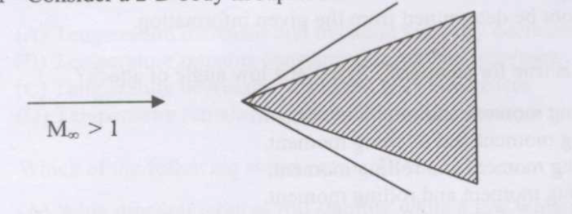
\includegraphics[width=0.8\textwidth]{figs/Gate1.png}
    \caption{}
    \label{}
\end{figure}
An increase in free stream Mach number $M_{\infty}$, will cause the oblique shock wave to
\begin{enumerate}
    \item move closer to the body
    \item move away from the body
    \item detach from the body
    \item become a normal shock
\end{enumerate}
\end{enumerate}
\end{document}

